% Projekt do Modelování a simulace
% Jan Šorm (xsormj00), Alena Tesařová (xtesar36), 2018
\documentclass[11pt,a4paper]{article}
\usepackage[utf8]{inputenc}
\usepackage[czech]{babel}
\usepackage[T1]{fontenc}
\usepackage{amsmath}
\usepackage{amsfonts}
\usepackage{amssymb}
\usepackage{fancyvrb}
\usepackage{float}
\usepackage{graphicx}
\usepackage{picture}
\usepackage{hyperref}
\usepackage[left=2cm,right=2cm,top=2.5cm,bottom=2cm]{geometry}
\author{Jan Šorm}
\begin{document}
\pagestyle{headings}
%%%%%%%%%%%%%%------------Titulni strana------------%%%%%%%%%%%%%%
\begin{titlepage}
	\begin{center}
		{\Huge\textsc{Vysoké učení technické v~Brně}}\\
		\medskip
		{\huge\textsc{Fakulta informačních technologií}}\\
		\vspace{\stretch{0.382}}
		{\LARGE Modelování a simulace}\\
		\medskip
		{\Huge Zadání č. 6 - Výroba piva}\\
		\vspace{\stretch{0.618}}
	\end{center}
	{\Large\today \hfill Šorm Jan, Tesařová Alena}
\end{titlepage}

\tableofcontents
\newpage

\section{Úvod}
Tato technická zpráva vznikla jako součást projektu do předmětu Modelování a simulace na škole Vysoké učení technické v Brně. V této zprávě je popsán simulační model \cite[str. 7]{pred} výroby piva ve společnosti Brněnská pivovarnická společnost s.r.o. \cite{pivo}. Důležitou součástí této zprávy jsou pak simulační experimenty, které slouží ke zjištění, zda nelze dosáhnout zefektivnění výroby.

\subsection{Autoři a zdroje informací}
Autory projektu jsou Jan Šorm a Alena Tesařová. Informace jsou čerpány z exkurze v pivovaru, které se zúčastnili oba autoři, osobního rozhovoru s panem Petrem Hauskrechtem po exkurzi a pozdější e-mailové korespondence se společností.

\subsection{Ověření validity modelu}
Většina našich informací pochází přímo od pana Hauskrechta, který je spoluvlastníkem společnosti a zároveň i dlouholetý sládek, takže by celý výrobní proces se všemi parametry měl být velmi přesný. Samotné výsledky našeho experimentu ohledně roční výroby, pak souhlasili s údaji, které nám sdělil pan Hauskrecht.

	
\section{Rozbor tématu a použitých metod} \label{sec:rozbor}
Tématem práce je simulace \cite[str. 8]{pred} výroby piva ve společnosti Brněnská pivovarnická společnost s.r.o. Pro výrobu piva jsou potřeba 4 základní ingredience: slad, voda, chmel a pivovarské kvasnice, které má pivovar vždy k dispozici. Výroba piva pak probíhá po várkách, kde z jedné várky se vyrobí 20 hl piva. Během jedné dvanáctihodinové směny pak proběhne pro jednu várku vystírání, rmutování, scezování, chmelovar a zchlazování a várka se přesune do kvasného tanku, kde začne probíhat několikadenní kvašení, než je tank připraven ke stáčení.

\subsection{Rmutování}
Při varném procesu dochází k rozšrotování sladu a smíchání s vodou, směs je ve varné nádobě a zahřeje se na teplotu 40-50 stupňů. Následně dochází ke rmutovacímu procesu, kdy proběhne rozštěpení škrobu na jednoduché cukry pomocí enzymům obsažených ve sladu. Používá se tzv. dvourmutový způsob rmutování, aby pivo dostalo svoji zlatavou barvu.

\subsection{Scezení}
Od odrmutování se musí oddělit sladina od nerozpustných součástí sladového mláta.

\subsection{Chmelovar}
Po skončení probíhá chmelovar, tzn. že se sladina vaří s přídavkem chmele, čímž se získá mladina. Mladina se zchladí na zákvasnou teplotu a čerpá se to kvasných tanků. 

\subsection{Kvašení}
Kvašení probíhá bez přístupu vzduchu, který by sebou nesl kvasinky, plísně, pyl a prachové částice a infikovat kvasící pivo. Kvasných tanků je celkem 23 o kapacitě 48 hl, takže do každého tanku se vlezou dvě várky a zbývající prostor je využit na pěnu. Jelikož je v tanku místo na dvě várky, tak se vždy vaří po sobě dvě várky stejného druhu piva. 

V pivovaru se vyrábí celkem 4 různé druhy piva. Každý druh se kvasí jinak dlouho a také tvoří jinačí procentuální zastoupení v celkové výrobě:
\begin{itemize}
\label{kvaseni}
  \item 10$^\circ$ -- 30 dní kvašení -- 13 \% celkové výroby
  \item 11$^\circ$ -- 35 dní kvašení -- 70 \% celkové výroby
  \item 12$^\circ$ -- 45 dní kvašení -- 10 \% celkové výroby
  \item 16$^\circ$ -- 90 dní kvašení -- 7 \% celkové výroby
\end{itemize}

Po skončení kvašení je celý tank připraven ke stáčení. 

Stáčení do sudů probíhá od pondělí do pátku denně a obsluhuje ho jedna směna. Stáčí se do sudů a z nich se následně stáčí do lahví a sklenic (celý proces trvá zhruba 6 hodin). Po každém vyprázdnění tanku je potřeba tank umýt, tento proces trvá 4 hodiny než je použitelný pro další plnění. Nová várka se začne dělat jen v případě, že existuje alespoň jeden čistý kvasný tank nebo tank, do kterého lze doplnit ještě jednu várku.

Směny na vaření jsou každý všední den dvě, v sobotu probíhá pouze denní a v neděli probíhá povinné čištění tanků na vaření. Směny na stáčení pak jsou jednou každý všední den.


\subsection{Použité postupy}
Pro tvorbu simulačního projektu byl použit jazyk C++ s knihovnou SIMLIB. Kromě toho, že použití knihovny simlib bylo doporučené již v samotném zadání projektu, poskytuje knihovna spoustu užitečných funkcí pro tvorbu simulačních modelů.

\subsection{Původ použitých postupů}
\begin{itemize}
\item C++ \url{https://cs.wikipedia.org/wiki/C%2B%2B}
\item Simlib \url{http://www.fit.vutbr.cz/~peringer/SIMLIB/} (GNU LGPL)
\item Demo cvičení IMS \url{http://perchta.fit.vutbr.cz/vyuka-ims/uploads/1/diskr2.pdf}
\end{itemize}

\section{Koncepce modelu}

\subsection{Zjednodušený model}
Cílem projektu bylo simulovat proces výroby piva a navrhnutí efektivnějšího systému výroby. Simulace se nezaměřuje na celý proces zpracování, ale pouze na část, kde se pivo vaří, leží v kvasných tancích a stáčí se. Vaření piva bude pro nás znamenat dobu, kdy dochází rmutování, scezení a chmelovaru pro jednoduchost.

\subsection{Odůvodnění vybrané části modelování}
V seznamu doby kvašení [\ref{kvaseni}] je uvedené, že doba kvašení není kratší než jeden měsíc. Zároveň pivovar disponuje pouze 23 tanky. Směny chodí do práce každý den včetně víkendů. Z těchto údajů plyne, že za nějakou dobu dojdou volné tanky a směny budou muset čekat než uběhne daná doba a tím pádem budou směny nevyužité. Tato myšlenka vedla k tomu, že jsme se zaměřili na zmíněnou část výroby.

\subsection{Popis konceptu}
Při modelování jsme postupovali nejprve tak, že jsme vytvořili abstraktní model, reprezentovaný stochastickou Petriho sítí [obr. \ref{fig:petri}], na základě informací v kapitole [\ref{sec:rozbor}].

%%% popis petriho site %%
V modelu máme jedinou linku s 23 tanky (na začátku uvažujeme, že jsou tanky prázdné). Do tanku se vejdou 2 uvařené várky, které vaří buď denní nebo noční směny (jedna směna uvaří jednu várku). Po naplnění tanku probíhá kvašení po dobu, která je závislá na druhu piva. Po uplynutí dané doby je tank připraven ke stáčení. Stáčení trvá 6 hodin. Po každém vyprázdnění tanku musí dojít k jeho čištění. Čištění jednoho tanku trvá 4 hodiny. Po každé desáté uvařené várce se musí tanky pořádně umýt, což trvá jednu celou směnu. Spodní část modelu značí příchod a odchod směn ze systému. Směny na vaření jsou každý pracovní den denní a noční. Víkendové směny jsou pouze ranní na vaření.

\begin{figure}[H]
  \centering
  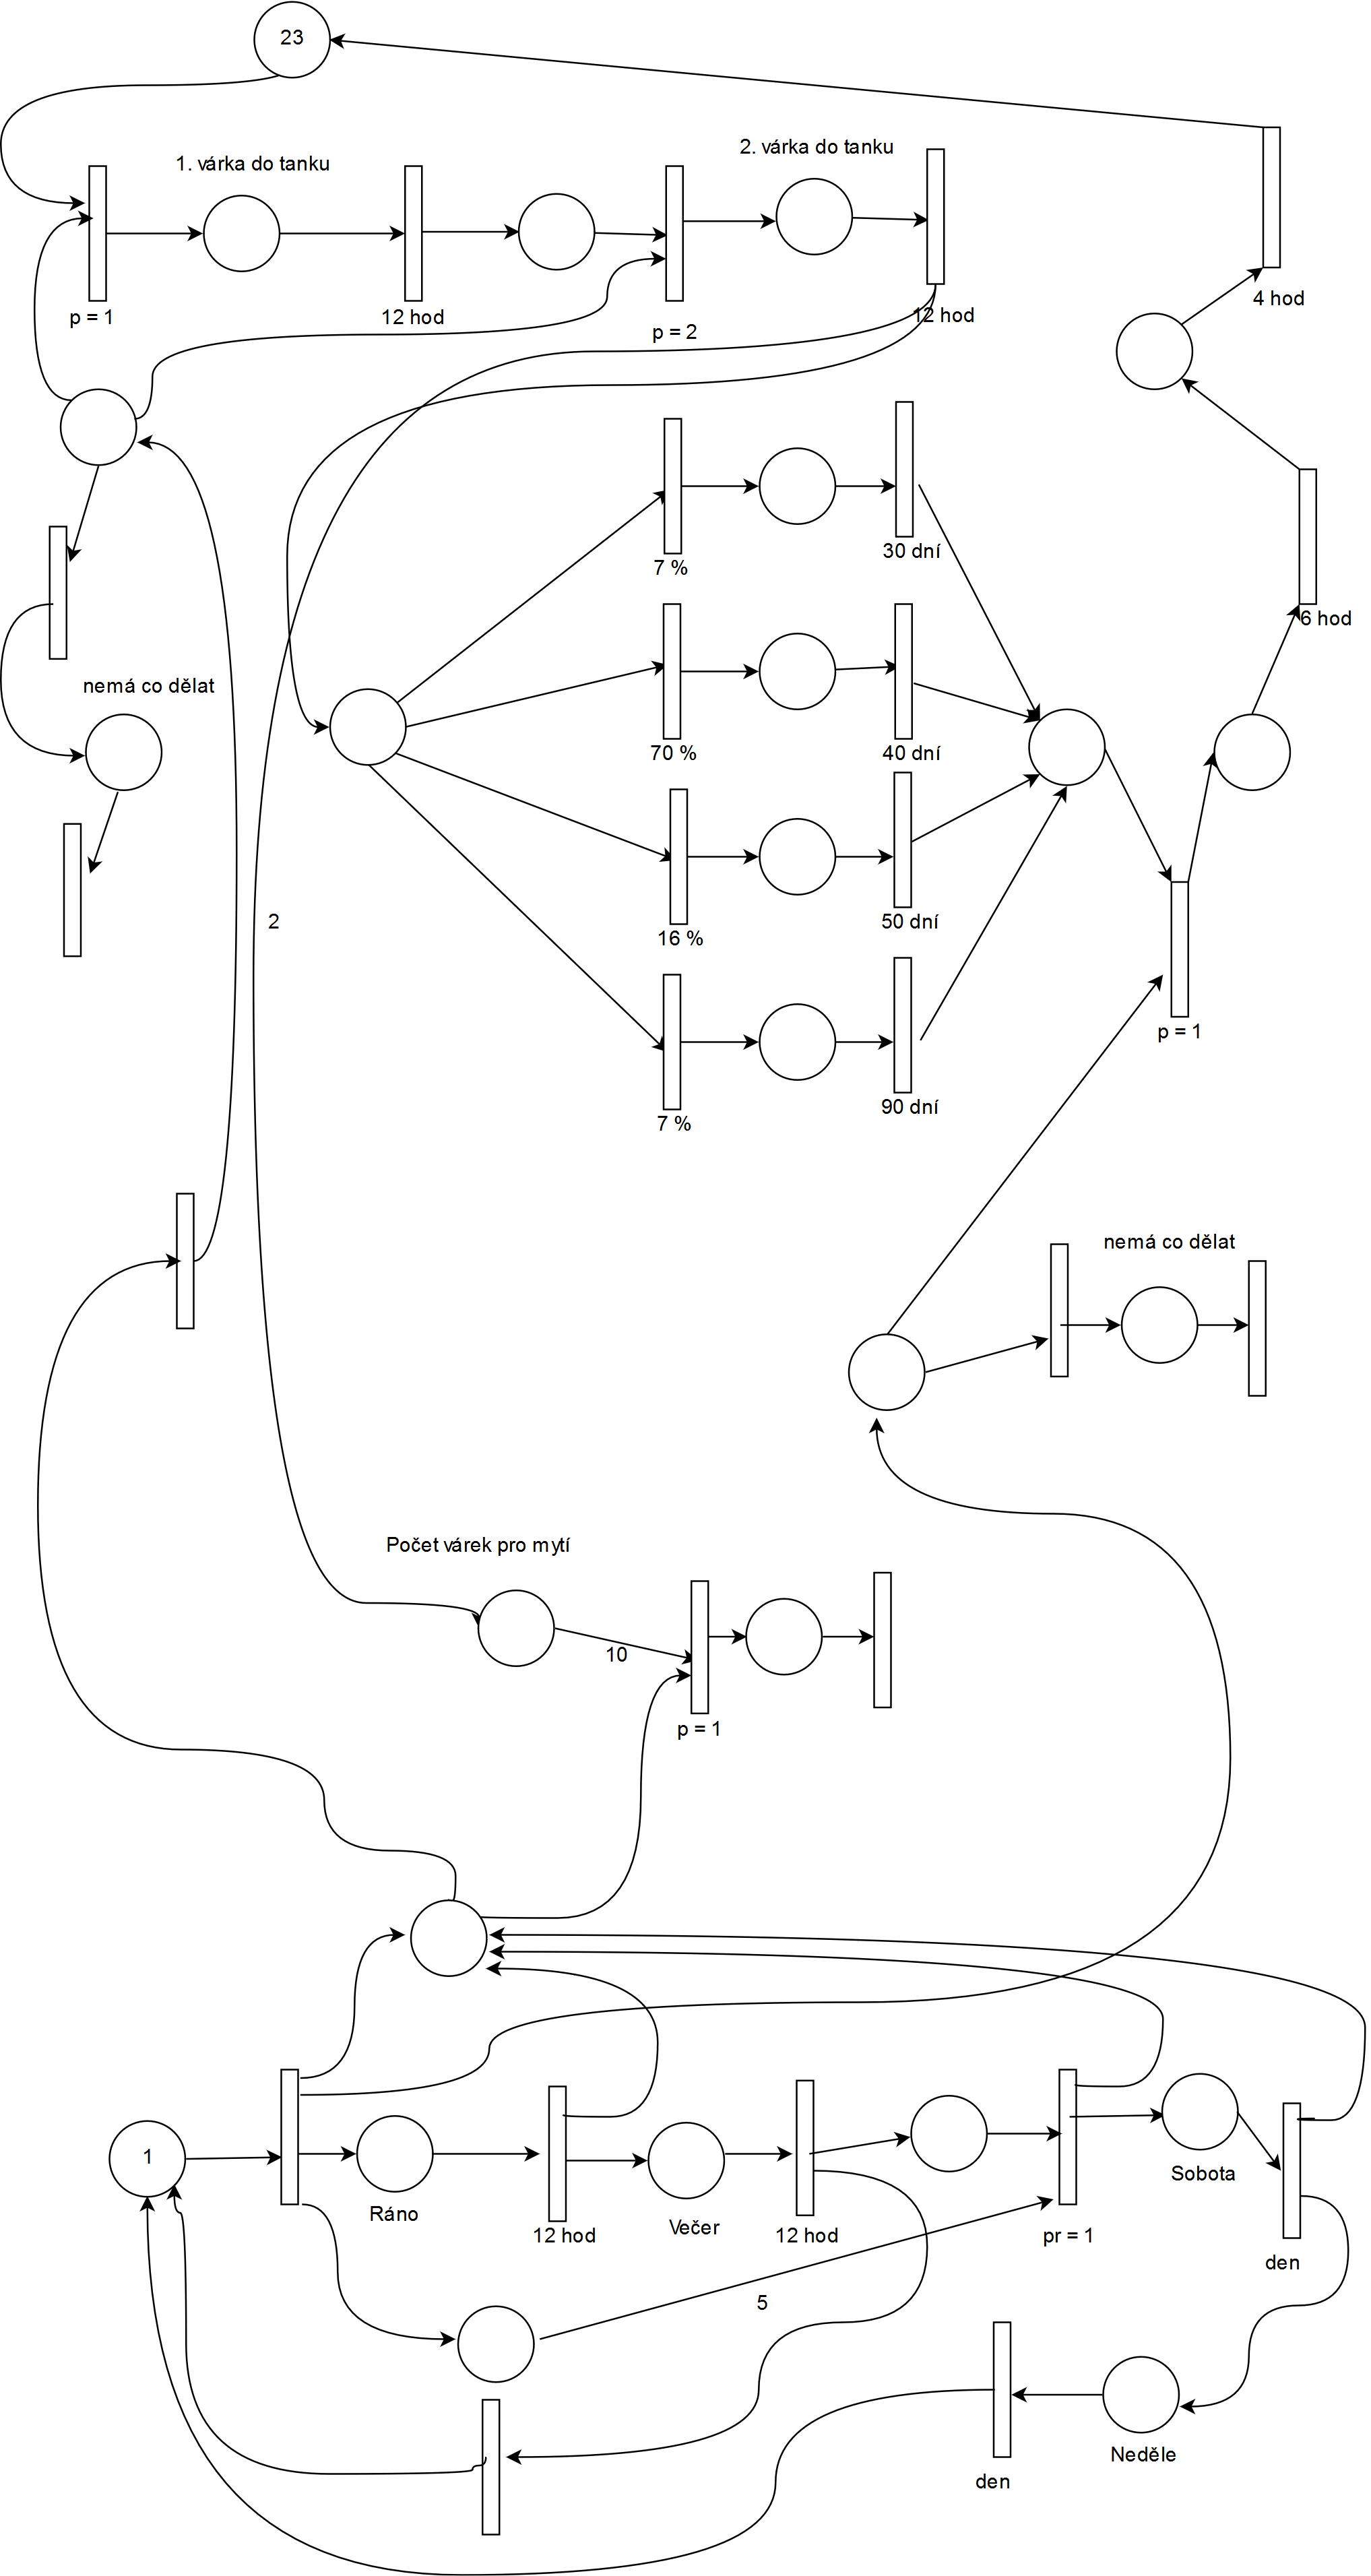
\includegraphics[width=15cm, height=25cm]{petri.png}
  \caption{Petriho síť znázorňující výrobu piva}
  \label{fig:petri}
\end{figure}

\section{Architektura simulačního modelu}


\section{Podstata simulačních experimentů a jejich průběh}
Cílem experimentů je zjistit, jakým způsobem lze docílit navýšení celkového množstvího vyrobeného piva za rok. Tento způsob je zaměřen především na navýšení počtu kvasných tanků, snížení počtu nevyužitých směn a případné zvýšení počtu směn o víkendu.

\subsection{Postup experimentování}
V prvním experimentu, který reprezentuje současný provoz pivovaru v průběhu deseti let, zjistíme referenční hodnoty. V následujících experimentech pak budeme vždy upravovat počet kvasných tanků a různě upravovat směny na stačení i na vaření.

\subsection{Průběh experimentů}
\subsubsection{Experiment 1}
V tomto experimentu je sledováno výchozí chování simulovaného modelu. Z naměřených hodnot v tomto experimentu bylo také potvrzeno, že simulace se chová věrohodně.

V tabulce \ref{tab:exp1} lze vidět data získaná ze simulace. Je v nich vidět první záběhový rok, v kterém je stočeno menší množství piva a směny bez práce se také liší od ostatních let. To je dáno tím, že na začátku jsou všechny kvasné tanky prázdné, první měsíc není tedy, co stáčet (tzn. zvýšené množství stáčecích směn bez práce a menší celkové množství stočeného piva) a naopak je pro každou vařící směnu volný tank k dispozici (tzn. snížený počet vařících směn bez práce).

Celkově pak jde vidět z naměřených dat, že se množství stočeného piva pohybuje každý rok okolo 7000 hl piva, což odpovídá zjištěné hodnotě v kapitole \ref{sec:rozbor}. Dále je také vidět velmi vysoký počet směn bez práce.
\begin{table}[h]
	\begin{center}
	\begin{tabular}{|r||r|r|r|}
	\hline
	\bfseries Rok & \bfseries Stočeno piva [hl] & \bfseries Vařící směny bez práce & \bfseries Stáčecí směny bez práce \\ \hline
	1 & 6520 & 218 & 98 \\ \hline
	2 & 7080 & 237 & 84 \\ \hline
	3 & 7120 & 233 & 83 \\ \hline
	4 & 6960 & 245 & 87 \\ \hline
	5 & 6960 & 243 & 87 \\ \hline
	6 & 7040 & 237 & 84 \\ \hline
	7 & 7040 & 237 & 84 \\ \hline
	8 & 7200 & 231 & 81 \\ \hline
	9 & 7000 & 242 & 86 \\ \hline
	10 & 7040 & 236 & 85 \\ \hline \hline
	\bfseries Celkem & \bfseries 69960 & \bfseries 2359 & \bfseries 859 \\ \hline
	\end{tabular}
	\caption{Data získaná ze simulace}
	\label{tab:exp1}
	\end{center}
\end{table}

\subsubsection{Experiment 2}
Tento experiment má za cíl zjistit, kolik je zapotřebí dokoupit kvasných tanků, abychom při zachování ostatních podmínek dosáhli největšího množství stočeného piva za deset let.

Z grafu \ref{fig:exp2tanky} vidíme, že optimální počet tanků je v tomto případě 37 (je tedy třeba dokoupit 14 kvasných tanků), při kterém se dosáhne množství 2571 stočených tanků za 10 let, což znamená 102 840 hl stočeného piva za deset let. Oproti výchozímu stavu (experiment 1) tedy dojde k navýšení výroby o 47 \%. Přidání dalšího tanku už pak nemá žádný efekt, což je vidět i v grafu \ref{fig:exp2smeny}, kde při 37 tancích klesne počet směn na stáčení, které jsou bez práce, na minimum.
\begin{figure}[H]
  \centering
  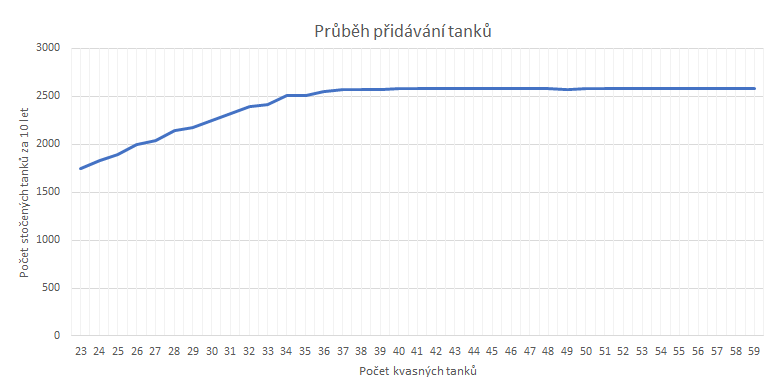
\includegraphics[width=15cm]{exp2tanky.png}
  \caption{Průběh přidávání tanků}
  \label{fig:exp2tanky}
\end{figure}

\begin{figure}[H]
  \centering
  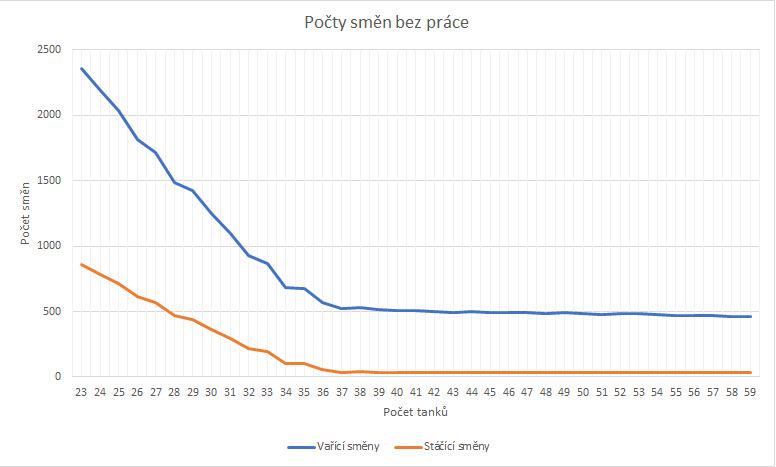
\includegraphics[width=15cm]{exp2smeny.png}
  \caption{Počty směn bez práce}
  \label{fig:exp2smeny}
\end{figure}


\subsubsection{Experiment 3}
Tento experiment má za cíl zjistit, kolik je zapotřebí dokoupit kvasných tanků při změněném počtu směn na stáčení (byly přidány nová směna v sobotu a v neděli), abychom při zachování ostatních podmínek dosáhli největšího množství stočeného piva za deset let.

Z grafu \ref{fig:exp3tanky} vidíme, že optimální počet tanků se v tomto případě zvýšil na 41 (je tedy třeba dokoupit celkem 18 kvasných tanků). Při tomto množství se dosáhne 2803 stočených tanků za 10 let, což znamená 112 120 hl stočeného piva za deset let. Oproti experimentu 2 tak dojde ke zvýšení o 9 \% a oproti experimentu 1 pak celkem o více jak 60 \%. Z pohledu na graf \ref{fig:exp3smeny} je pak vidět, že máme velmi vysoký počet směn na stáčení, což se pokusíme snížit následujícím experimentem.

\begin{figure}[H]
  \centering
  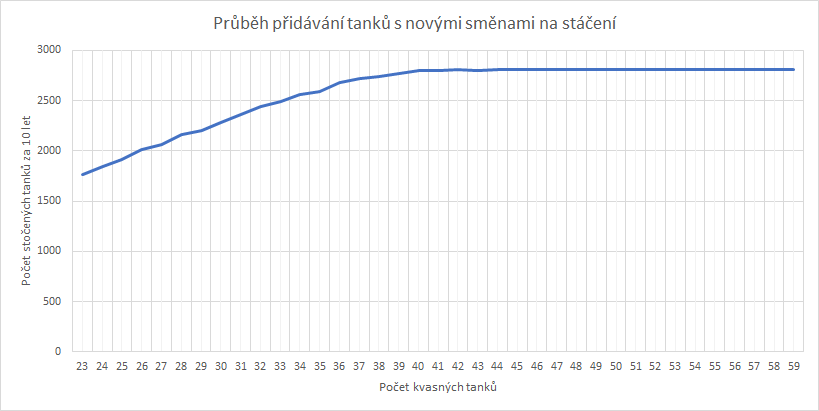
\includegraphics[width=15cm]{exp3tanky.png}
  \caption{Průběh přidávání tanků}
  \label{fig:exp3tanky}
\end{figure}

\begin{figure}[H]
  \centering
  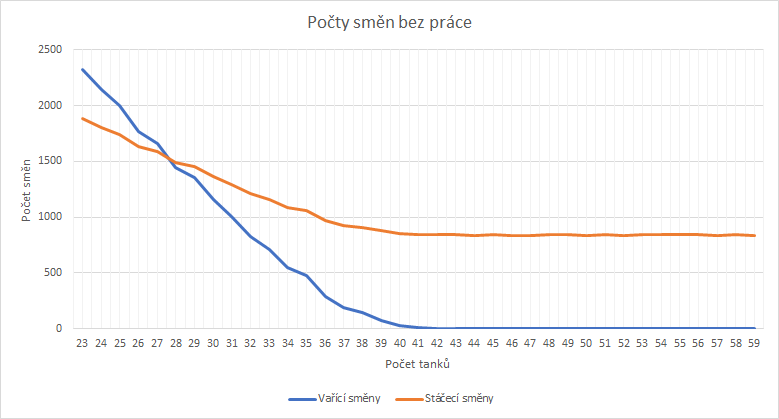
\includegraphics[width=15cm]{exp3smeny.png}
  \caption{Počty směn bez práce}
  \label{fig:exp3smeny}
\end{figure}

\subsubsection{Experiment 4}
Tento experiment má za cíl zjistit, kolik je zapotřebí dokoupit kvasných tanků při změněném počtu směn na stáčení (tak jak je popsáno v experimentu 3) a při změněném počtu směn na vaření (byly přidány noční směny v sobotu a v neděli), abychom při zachování ostatních podmínek dosáhli největšího množství stočeného piva za deset let.

Z grafu \ref{fig:exp4tanky} vidíme, že optimální počet tanků je v tomto případě 47 (je tedy třeba dokoupit celkem 24 kvasných tanků). Při tomto množství se dosáhne 3277 stočených tanků za 10 let, což znamená 131 080 hl stočeného piva za deset let. Oproti experimentu 3 tak dojde ke zvýšení o téměř 17 \% a oproti experimentu 1 pak celkem o více jak 87 \%. Z pohledu na graf \ref{fig:exp4smeny} je pak vidět, že se o proti experimentu 3 počet směn na stáčení zmenšil o polovinu.

\begin{figure}[H]
  \centering
  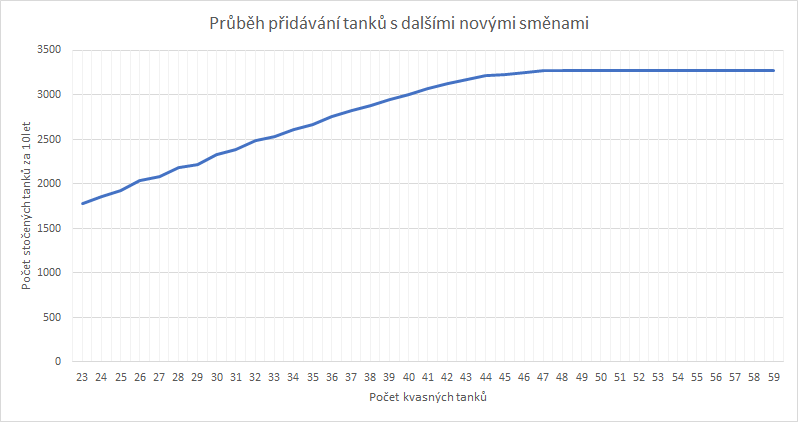
\includegraphics[width=15cm]{exp4tanky.png}
  \caption{Průběh přidávání tanků}
  \label{fig:exp4tanky}
\end{figure}

\begin{figure}[H]
  \centering
  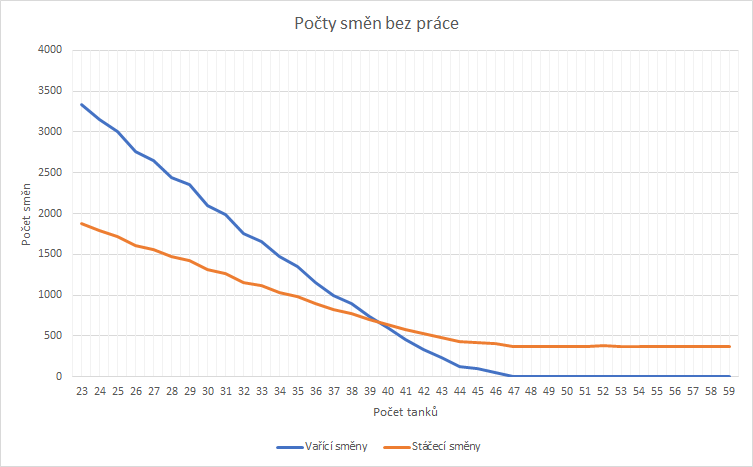
\includegraphics[width=15cm]{exp4smeny.png}
  \caption{Počty směn bez práce}
  \label{fig:exp4smeny}
\end{figure}

\subsection{Závěry experimentů}
Byly provedeny celkem 4 experimenty, z nichž první sloužil k ověření věrohodnosti modelu a získání referenčních hodnot a zbývající tři se pak zaměřovali na zjištění optimálního počtu kvasných tanků při různě změněných podmínkách a celkového množství piva vyrobeného za 10 let.

Další možnosti přidávání směn na vaření už nelze provádět, jelikož už byly vyčerpány všechny volné časové období během týdne. Bylo by tak potřeba přidat novou linku na vaření, což už by byl ale příliš velký zásah do současných možností pivovaru.
   
\section{Shrnutí simulačních experimentů a závěr}
Na základě hodnot získaných z experimentu 1 a porovnání s informacemi od pana Hauskrechta došli autoři k závěru, že se navržený systém chová věrohodně.

Dle experimentu 2 bylo zjištěno, že při pouhém zvýšení současného počtu kvasných tanků na 37 dojde ke zvýšení výroby piva o 47 \%.

Na základě hodnot zbylých dvou experimentů pak bylo zjištěno, že při počtu 47 tanků (tzn. zdvojnásobení současného počtu a přidání ještě jednoho tanku) dojde ke zvýšení výroby piva o 87 \% a to při přidání dvou směn na stáčení a dvou směn na vaření (tzn., že o víkendech by probíhaly směny stejně jako ve všední dny).


   
\newpage
\begin{thebibliography}{Per00}
	\bibitem[1]{pred} Peringer P., Hrubý M.:
    \emph{Modelování a simulace [online]. [vid. 5. prosince 2018]. Dostupné z: https://www.fit.vutbr.cz/study/courses/IMS/public/prednasky/IMS.pdf }
	\bibitem[2]{simlib} Peringer P.:
    \emph{SIMLIB/C++ [online]. [vid. 5. prosince 2018]. Dostupné z: http://www.fit.vutbr.cz/\~{}peringer/SIMLIB/ }
	\bibitem[3]{pivo} \emph{Brněnská pivovarnická společnost s.r.o. [online]. [vid. 5. prosince 2018]. Dostupné z: https://www.hauskrecht.cz/ }
\end{thebibliography}
	
\end{document}
